%% Los cap'itulos inician con \chapter{T'itulo}, estos aparecen numerados y
%% se incluyen en el 'indice general.
%%
%% Recuerda que aqu'i ya puedes escribir acentos como: 'a, 'e, 'i, etc.
%% La letra n con tilde es: 'n.

\chapter{Métodos}
%\setcounter{section}{1}
\section{Métodos estadísticos}

\subsection{Modelo AMMI y SREG}

El modelo AMMI propuesto por Zobel et al. (1988) es un modelo multiplicativo en el cual se expresa el fenotipo de un genotipo en un ambiente de la siguiente forma:
\begin{center}
$y_{ij}= \mu +G_i + A_j + \sum_{k=1}^q \lambda_k \alpha_{ik} \gamma_{jk}$ \hspace{0.5cm} $ i=1,...,g$;\hspace{0.15cm} $ j=1,...,a$;\hspace{0.15cm} $q=min(g-1,a-1)$
\end{center} 
donde 
\begin{itemize}
\item $y_{ij}$ es el caracter fenotípico evaluado (rendimiento o cualquier otro caracter de interes) del $i$-ésimo genotipo en el $j$-ésimo ambiente,
\item $\mu$ es la media general,
\item  $G_i$ es el efecto del $i$-ésimo genotipo,
\item $A_j$ es el efecto del $j$-ésimo ambiente
\item $\sum_{k=1}^q \lambda_k \alpha_{ik} \gamma_{jk}$ es la sumatoria de componentes multiplicativas utilizadas para modelar la IGA. Siendo, $\lambda_k$ el valor singular para la  $k$-ésima componente principal (PC) $\alpha_{ik}$ y $\gamma_{jk}$ son los scores de las PC para el $i$-ésimo genotipo y el $j$-ésimo ambiente para la $k$-ésima componente, respectivamente.
\end{itemize}

En cambio, el modelo SREG (Cornelius et al., 1996; Crossa y Cornelius, 1997 y 2002) expresa el fenotipo de un genotipo en un ambiente en función del efecto ambiente aditivo y los efectos genotipo e interacción agrupados y en forma multiplicativa:
\begin{center}
$y_{ij}= \mu +  A_j + \sum_{k=1}^q \lambda_k \alpha_{ik} \gamma_{jk}$ \hspace{0.5cm} $ i=1,...,g$;\hspace{0.15cm} $ j=1,...,a$; \hspace{0.15cm} $q=min(g-1,a)$
\end{center} 

Los parámetros multiplicativos, tanto en el modelo AMMI como en el SREG, se estiman por medio de la Descomposición en Valores Singulares (DVS) de la matriz que contiene los residuos del modelo aditivo luego de ajustar por mínimos cuadrados el modelo de efectos principales. Generalmente los dos primeros términos multiplicativos son suficientes para explicar los patrones de la IGA o de G e IGA en forma conjunta; la variabilidad remanente se interpreta como ruido. 

Para visualizar el efecto de IGA o conjuntamente el de G e IGA se proponen los gráficos biplots GE (\emph{Genotipe-Environment}) (\textbf{CITA}) y GGE (\emph{Genotipe} plus \emph{Genotipe-Environment}) (Yan et al., 2000) respectivamente. El concepto del biplot fue presentado por Gabriel (1971), consiste en la representación de las filas (individuos) y las columnas (variables) de una matriz de datos en un mismo gráfico. Éstos biplots, son herramientas poderosas para el análisis e interpretación de la estructura de datos provenientes de ensayos multiambientales utilizados en los programas de mejoramiento (Ebdon y Gauch, 2002; Samonte et al., 2004; Yan et al., 2000; Zobel et al., 1988).

El biplot GE ayuda a interpretar la variación producida por los efectos de la IGA; mientras que en el biplot GGE se analizan conjuntamente el efecto de G+IGA. Para seleccionar cultivares, el efecto de G e IGA debe considerarse simultáneamente. Por esta razón, el modelo SREG es superior a AMMI para visualizar patrones en datos MET. El biplot GGE permite investigar la existencia de megaambientes (grupo de ambientes en donde los cultivares de mejor desempeño son los mismos) entre los ambientes en estudio, seleccionar cultivares superiores en un megaambiente dado y seleccionar los mejores ambientes de evaluación para analizar las causas de la IGA.

\textbf{Hablar un poco de los metodos de SVD del modelo SREG que da lugar a distintos graficos. Un oracion tipo dependiendo del escalado utilizado se pueden obtener distintas interpretaciones....}

\subsection{Modelo AMMI robusto}

El modelo AMMI, en su forma estándar, asume que no hay valores atípicos en el conjunto de datos. La presencia de \emph{outliers} es más una regla que una excepción cuando se consideran datos agronómicos debido a errores de medición, algunas plagas / enfermedad que puede influir en algunos genotipos  resultando por ejemplo en un rendimiento inferior al esperado en un ambiente, o incluso debido a alguna característica inherente de los genotipos que se evalúan.

Rodrigues et al. (2015) proponen una generalización robusta del modelo AMMI, que resulta de ajustar la regresión robusta basada en el estimador M-Huber (Huber, 1981) y luego utilizar un procedimiento DVS / PCA robusto. Consideraron varios métodos de DVS / PCA dando lugar a un total de cinco modelos robustos llamados: R-AMMI, H-AMMI, G-AMMI, L-AMMI, PP-AMMI. 

El empleo de la versión robusta del modelo AMMI puede ser extremadamente útil debido a que una mala representación de genotipos y ambientes en los biplots puede dar como resultado un mala decisión con respecto a qué genotipos seleccionar para un conjunto dado de ambientes (Gauch1997,Yanetal2000). A su vez, la elección de los genotipos incorrectos pueden provocar grandes pérdidas en términos de rendimiento. Los biplots obtenidos de los modelos robustos mantienen las características e interpretación estándar del modelo AMMI clásico (Rodrigues et al. (2015)).


\subsection{Métodos de imputación}


Una limitación importante que presentan los modelos multiplicativos descriptos previamente es que requieren que el conjunto de datos este completo, es decir no admiten valores perdidos. Aunque los EMA están diseñados para que todos los genotipos se evalúen en todos los ambientes, la presencia de valores faltantes es muy común debido a errores de medición o pérdidas de plantas por animales, inundaciones o problemas durante la cosecha, además de la dinámica propia de la evaluaciones en las que se incorporan y se descartan genotipos debido a su pobre desempeño (Hill y Rosemberg, 1985)

Se han propuesto numerosas metodologías para superar el problema de valores ausentes en el conjunto de datos, entre las cuales se encuentran:

\begin{itemize}
\item EM-AMMI: Gauch y Zobel (1990) desarrollaron un procedimiento iterativo que utiliza el algoritmo de maximización de la esperanza (EM, del inglés \emph{Expectation-Maximization}) incorporando el modelo AMMI. 
\end{itemize}
\begin{itemize}
\item EM-SVD: Perry (2009a) propone un método de imputación que combina el algoritmo EM con DVS. 
\end{itemize}
\begin{itemize}
\item EM-PCA: Josse y Husson (2013) proponen imputar los valores faltantes de un conjunto de datos con el modelo de Análisis de componentes principales.
\end{itemize}
\begin{itemize}
\item Gabriel Eigen: Arciniegas-Alarcón et al. (2010) propuso un método de imputación que combina regresión y aproximación de rango inferior usando DVS. 
\end{itemize}
\begin{itemize}
\item WGabriel Eigen:
\end{itemize}




\section{Paquete de R}

%https://oscarperpinan.github.io/R/Paquetes.html 
En R, la unidad fundamental de código que se puede compartir es el paquete. Éste agrupa códigos, datos, documentación y pruebas, y es fácil de compartir con otros. Para crear uno de ellos, se deben seguir los siguientes pasos, teniendo en cuenta que en cada uno de ellos se debe probar la presencia de errores:

\begin{itemize}
\item Crear la estructura del paquete.
\item Incluir funciones y conjuntos de datos.
\item Redactar la documentación.
\item Pruebar el flujo de trabajo.
\item Compilar e instalar.
\item Publicar.
\end{itemize}

\textbf{Quisiera poner algo como que no es un camino lineal, sino que cada cosa que se hace se debe chequear y se va a otro paso y se chequea nuevamente, etc... incluso en la parte de publicación, se crea el readme y se chequea}

Para el desarrollo del mismo se utilizan numerosas funciones incluidas en el paquete \emph{devtools} \citep{Hadley2019} ya que facilita el proceso de creación del mismo, \emph{roxygen2} para redactar la documentación, \emph{testthat} a fin de probar el flujo de trabajo y \emph{knitr} para generación de informes dinámicos. Antes de comenzar, se debe contar con la última versión de R, con una versión reciente del IDE de RStudio y cargar los paquetes mencionados en la sesión de trabajo. 



\subsection{Creación de la estructura}

Para crear la estructura del paquete se utiliza la función \textcolor{blue}{create\_package}(). El principal y único argumento requerido por dicha función es el directorio donde el nuevo paquete se alojará. Por lo general, si el directorio se llama ``geneticae'', entonces el nombre del paquete también será ``geneticae'':


\begin{lstlisting}
# Cargar la libreria devtools
library(devtools)
# Crear el paquete geneticae
create_package(``C:/Users/Julia/Desktop/geneticae")
\end{lstlisting}


El resultado de ejecutar dicha función es un paquete con los siguientes componentes:
\begin{itemize}
\item Un directorio R/.
\end{itemize}
\begin{itemize}
\item DESCRIPTION, un archivo simple cuyo objetivo es almacenar metadatos importantes sobre el paquete, epecifica el título, la versión del mismo, identifica al autor y brinda un mail de contacto, una breve descripción del paquete, la lista de los paquetes que el paquete creado necesita para funcionar, la licencia, entre otros.

El contenido básico en un archivo DESCRIPTION es:
\end{itemize}

\begin{verbatim}
Package: geneticae
Title: What the Package Does (One Line, Title Case)
Version: 0.0.0.9000
Authors@R: 
    person(given = "First",
           family = "Last",
           role = c("aut", "cre"),
           email = "first.last@example.com",
           comment = c(ORCID = "YOUR-ORCID-ID"))
Description: What the package does (one paragraph).
License: What license it uses
Encoding: UTF-8
LazyData: true
\end{verbatim}




\begin{itemize}
\item Un archivo NAMESPACE
\end{itemize}

Los archivos y el directorio R/ se irán modificando a medida que el paquete se vaya creando. Además se crearán los siguientes archivos: geneticae.Rproj, proyecto de RStudio que hace que el paquete sea fácil de usar con RStudio; .Rbuildignore enumera los archivos que se necesitan, pero que no deben incluirse al compilar el paquete y .gitignore anticipa el uso de Git.




\subsection{Inclusión de funciones y de conjuntos de datos}

Una vez creada la estructura del paquete se deben incluir las funciones que el mismo contendrá. Cada una de ellas debe ser guardada en un archivo de extensión .R, en el subdirectorio R/. Para ello, se utiliza la función \textcolor{blue}{use\_r}() la cual crea y/o abre un script de la carpeta R/.

Una vez creada una función, se realizan pruebas para asegurar que el código realice lo que realmente se desea utilizando la función \textcolor{blue}{load\_all}() que simula el proceso de construcción, instalación y conexión del paquete. Permite que las funciones creadas estén disponible rápidamente para uso interactivo, del mismo modo que si se hubiera construido e instalado el paquete y luego cargada en la sesión de R a través de la función \textcolor{blue}{library}(geneticae).

Muy frecuentemente se utilizan funciones que se encuentran disponibles en otros paquetes. En algunos casos solo se utilizan unas pocas funciones de otro paquete, por lo tanto con la función \textcolor{blue}{use\_package}() se agrega el paquete de interés a la sección Imports del archivo DESCRIPTION, y luego para llamar a las mismas se utiliza paquete::función. Si las funciones de otro paquete son utilizadas reiteradamente resulta conveniente utilizar, @importFrom paquete función. Esto tiene un pequeño beneficio de rendimiento, ya que :: agrega mayor tiempo de evaluación a la función. Alternativamente, si está utilizando repetidamente muchas funciones de otro paquete, puede importarlas todas utilizando @import paquete. Esta es la solución menos recomendada porque hace que su código sea más difícil de leer (no se puede saber de dónde proviene una función), y si @import tiene muchos paquetes, aumenta la posibilidad de que entren en conflicto nombres de funciones.

A menudo es útil incluir datos en un paquete a fin de proporcionar ejemplos de aplicaciones de las funciones incluidas en él. Ellos se almacenan en el directorio data/, siendo cada archivo un .RData que sólo contiene un objeto. Para esto, se utiliza la función \textcolor{blue}{usethis::use\_data}(). Notar que el archivo DESCRIPTION creado con la función \textcolor{blue}{create\_package}(), mencionada anteriormente, contiene el campo LazyData: true, lo cual genera que los conjuntos de datos no ocupen memoria hasta que sean usados.

\subsection{Documentación}

Uno de los aspectos más importantes del paquete es la documentación ya que le indica a los usuarios cómo se deben usar las funciones incluidas. Existen múltiples formas de documentar un paquete, la forma estándar es escribir archivos con extensión .Rd, los cuales utilizan una sintaxis basada en LaTeX, en la carpeta man. Sin embargo, el paquete \emph{roxygen2}, utilizado en este trabajo, convierte los comentarios con formato especial en archivos .Rd. Esta última forma de documentación proporciona una serie de ventajas sobre la forma estándar entre las cuales se encuentra que el código y la documentación son adyacentes, de modo que cuando el código se modifique le exigirá que actualice la documentación. 

El flujo de trabajo para crear la documentación con el paquete \emph{roxygen2} es el siguiente:

\begin{itemize}
\item Agregar comentarios a los archivos .R. Estos deben comenzar con \#', para distinguirlo de los comentarios regulares, y preceden a una función. La primera oración se convierte en el título y el segundo párrafo es una descripción de la función. Seguidamente se utilizan las siguientes etiquetas para completar la documentación:

\begin{itemize}
\item @param describe los parámetros de la función, indica de que clase es el parámetro y para que sirve.
\item @examples proporciona un código ejecutable que muestra cómo usar la función en la práctica. 
\item @return describe el resultado de la función. 
\end{itemize}

\item Ejecutar devtools::document() para convertir los comentarios de roxygen en archivos .Rd. 
\end{itemize}

\emph{Roxygen2} permite utilizar la descripción de los parámetros de otras funciones usando @inheritParams. Esta documentará los parámetros que no están documentados en la función actual, pero que si lo están en la función fuente. La fuente puede ser una función en el paquete actual, vía @inheritParams function, u otro paquete, vía @inheritParams package::function. Además \emph{Roxygen2} permite incluir referencias utilizando @references.

A diferencia de las funciones que son documentadas directamente, para los objetos en data/, se debe crear un archivo y guardarlo en el directorio R/.\\

\textbf{Viñetas}

A diferencia de la documentación, en la cual se detalla como se utiliza cada una de las funciones del paquete, una viñeta es una descripción el problema que el paquete está diseñado para resolver y muestra al lector cómo resolverlo.

Muchos de los paquetes existentes tienen viñetas la cuales se pueden encontrar utilizando la función \textcolor{blue}{browseVignettes}(``packagename") si el mismo se encuentra instalado, sino deben consultarse en su página de CRAN, por ejemplo para el paquete \emph{dplyr}: \url{http://cran.r-project.org/web/packages/dplyr}. Cada viñeta proporciona el archivo fuente original, una página HTML o PDF y un archivo de código R. 

Las Viñetas se pueden construir de diversas formas, en este trabajo se utiliza se utiliza \textcolor{blue}{usethis::use\_vignette}(``my-vignette''). La misma crea un directorio vignettes/, agrega las dependencias necesarias a DESCRIPTION y redacta la viñeta. Las tres componentes fundamentales de la misma son las siguientes:

\begin{itemize}
\item El bloque inicial de metadatos, que contiene la siguiente información:
\end{itemize}

\begin{verbatim}
---
title: "Vignette Title"
output: rmarkdown::html_vignette
vignette: >
  %\VignetteIndexEntry{Vignette Title}
  %\VignetteEngine{knitr::rmarkdown}
  \usepackage[utf8]{inputenc}
---
\end{verbatim}

\begin{itemize}
\item Markdown para formatear texto.
\item Knitr para interpretar texto, código y resultados.
\end{itemize}

\subsection{Pruebas del flujo de trabajo}

Las pruebas resultan fundamentales en el desarrollo de paquetes, asegura que el código haga lo que realmente se desea. Existen pruebas informales como aquellas realizadas con la función \textcolor{blue}{load\_all}() que permite que las funciones creadas estén disponible rápidamente para uso interactivo. Sin embargo, las pruebas interactivas pueden convertirse en scripts reproducibles, los cuales resultan superiores debido a que se indica explícitamente cómo debería comportarse el código, provocando que los errores solucionados no vuelvan a ocurrir.

Por lo tanto, en lugar de \textcolor{blue}{load\_all}(), se utiliza la función \textcolor{blue}{usethis::usetestthat}() (Wickham,2011). Esta crea un directorio tests/testthat, agrega testthat al campo Suggests en el archivo DESCRIPTION y además, crea un archivo tests/testthat.R.  

Las pruebas se organizan jerárquicamente: una expectativa describe el resultado esperado de un cálculo, cada prueba agrupa múltiples expectativas para probar la salida de una función y un archivo agrupa múltiples pruebas relacionadas.


Existen tres formas de llevar a cabo las pruebas:
\begin{itemize}
\item Ejecutar todas las pruebas en un archivo o directorio \textcolor{blue}{test\_file}() o \textcolor{blue}{test\_dir}().
\item Ejecutar pruebas automáticamente cada vez que algo cambie con la función \textcolor{blue}{autotest}(). Estas son útiles cuando las pruebas se ejecutan con frecuencia. Si se modifica un archivo de prueba, probará ese archivo; si se modifica un archivo de código, volverá a cargar ese archivo y volverá a ejecutar todas las pruebas.
\item Hacer que R CMD check ejecute sus pruebas.
\end{itemize}


\subsection{Compilación e instalación}

La función \textcolor{blue}{check}() o R CMD check ejecutado en el shell, es utilizado para verificar que un paquete R esta en pleno funcionamiento. La misma verificará que no haya errores de sintaxis o no se generen warnings. Está compuesto por más de 50 chequeos individuales entre los cuales se encuentran: la estructura del paquete, el archivo descripción, namespace, el código de R, los datos, la documentación, entre otros. Se aconseja realizar verificaciones completas de que todo funciona a medida que se van incorporando funciones ya que si se incorporan muchas y luego se verifican será dificil identificar y resolver los problemas. Una vez que no se detectan errores, advertencias o notas, se ejecuta la función \textcolor{blue}{install}(), con el objetivo de instalar el paquete en la biblioteca.


\subsection{Publicación}
%https://rsanchezs.gitbooks.io/ciencia-de-datos-con-r/paquetes/paquetes.html
Un repositorio es el lugar dónde se encuentran alojados los paquetes y desde el cuál los usuarios pueden descargarlos. Entre los repositorios más populares de paquetes R se encuentran:

\begin{itemize}
\item \textbf{CRAN}: es el principal repositorio de paquetes de R, está coordinado por la fundación R. Previa a la publicación en este repositorio el paquete debe pasar por diferentes pruebas para asegurar que cumple con las políticas de CRAN.

\item \textbf{Bioconductor}: se trata de un repositorio específico para bioinformática. Del mismo modo que CRAN, tiene sus propias políticas de publicaciones y procesos de revisión.

\item \textbf{GitHub}: a pesar que no es específico para R, github es con toda seguridad el repositorio más popular para la publicación de proyectos \emph{open source} (del inglés, código abierto). Su popularidad procede del espacio ilimitado que proporciona para el alojamiento de proyectos \emph{open source}, la integración con git (un software de control de versiones) y, la facilidad de compartir y colaborar con otras personas. Una de sus desventajas es que no proporciona procesos de control.

\item \textbf{R-Forge} y \textbf{RForge}: son entornos de desarrollo de paquetes y repositorios. Eso significa que incluyen control de fuente, seguimiento de errores y otras características. Puede obtener versiones de desarrollo de paquetes de estos.
\end{itemize}

El paquete \emph{geneticae} se encuentra en GitHub, para instalar el mismo se deben seguir las siguientes instrucciones:

\begin{lstlisting}
library(devtools)
install_github(``jangelini/geneticae") 
\end{lstlisting}


Una vez que el paquete se carga en GitHub, resulta importante crear y modificar el archivo README.md ya que constituye la página de inicio del paquete. El objetivo principal de este archivo es responder a las siguientes preguntas sobre el paquete: ¿Por qué debería usarlo?, ¿Cómo lo uso? y ¿Cómo lo consigo?. En GitHub, README.md se representará como HTML y se mostrará en la página de inicio del repositorio. Para generar el readme con R Markdown se utiliza la función \textcolor{blue}{use\_readme\_rmd}() la cual crea una plantilla README.Rmdy la agrega a .Rbuildignore.

Por otro lado, se crea también una página web\footnote{Para visitar la página web del paquete debe dirigirse a \url{https://...........}} para el paquete utilizando \emph{pkgdown}, mediante la función \textcolor{blue}{pkgdown::build\_site}(). En ella se podrá encontrar una breve descripción del paquete, las funciones que incluyen los mismos, la vignette, las distintas versiones del paquete, entre otras cosas.  


\section{Shiny APP}
Shiny es un paquete R para crear aplicaciones web interactivas sin necesidad de conocer en profundidad los lenguajes HTML / CSS / JavaScript . Estas aplicaciones constituyen una interfaz gráfica entre el usuario y R, que permiten realizar un análisis a través de un navegador web sin necesidad de programar.

El esquema interno de una Shiny APP puede observarse en la Figura \ref{fig:fig321}. Las mismas están compuestas por la interfaz de usuario, ui (\emph{user interfaz}), que controla el diseño de la aplicación, recibe los inputs y muestra los outputs en el navegador; el server que contiene las funciones de R con las instrucciones neesarias para obtener los resultados de los análisis incluidos en la aplicación; y shinyApp es la función que crea objetos de aplicación Shiny a partir de ui / servidor. 

\begin{figure}[H]
\begin{center}
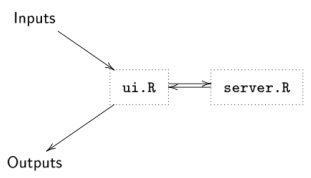
\includegraphics[width=7cm]{./Graficos/figura7}
\end{center}
\caption{Esquema interno de la aplicación.}
\label{fig:fig321}
\end{figure}


\subsection{Desarrollo de Shiny APP}

Una forma de desarrollar una  aplicación es a partir de un nuevo directorio con un sólo archivo llamado app.R, como se muestra a continuación. 

\begin{lstlisting}
library(shiny)
ui<- ...
server<- ...
shinyApp(ui = ui, server = server)
\end{lstlisting}

En este archivo se carga el paquete shiny, se define la interfaz de usuario y la función server y por último, se ejecuta función que permite construir e iniciar una aplicación. Al ejecutar la aplicación la misma aparecerá, de manera predeterminada, en una ventana emergente. Sin embargo, otras dos opciones se pueden configurar desde el menú desplegable de \emph{Run App}. Una de ellas es la ejecución en el panel del visor que permite verla al mismo tiempo que ejecuta el código. La segunda opción es ejecutar en un navegador externo mostrando la aplicación como la mayoría de los usuarios la verán. Dado que la sesión de R estará monitoreando la aplicación y ejecutando las ordenes dadas por el usuario, no se podrá ejecutar ningún comando.

En cualquier lenguaje de programación tener el código duplicado genera un desperdicio computacional y, lo que es más importante, aumenta la dificultad de mantener o depurar el código. Cuando se programa en R, se utilizan dos técnicas para lidiar con el código duplicado: guardar un valor usando una variable o utilizar una función para almacenar un cálculo. Ninguno de estos enfoques son apropiados en una Shiny APP, sino que se utilizan expresiones reactivas. Una expresión reactiva tiene una diferencia importante con una variable: sólo se ejecuta la primera vez que se llama y luego almacena en caché el resultado de la misma hasta que necesite actualizarse. La programación reactiva es un estilo de programación que enfatiza valores que cambian con el tiempo, y cálculos y acciones que dependen de esos valores. Esto es importante para las aplicaciones Shiny porque son interactivas: los usuarios cambian los inputs, lo que hace que la lógica se ejecute en el servidor que finalmente resultan en actualización de los outputs/resultados.

Entre los problemas que pueden surgir al crear una Shiny app se encuentran los errores inesperados, no se obtiene ningún error pero el valor obtenido es incorrecto, o bien todos los resultados son correctos, pero no se actualizan cuando se deben. Una vez localizada la fuente del error, la herramienta más poderosa es el depurador interactivo, éste detiene la ejecución y brinda una consola interactiva donde puede se ejecutar cualquier código para descubrir el error. Para iniciar el mismo, se puede agregar la función browser() en el código fuente, o bien agregar un punto de interrupción RStudio haciendo clic a la izquierda del número de línea.

Al modificar la aplicación, se la ejecuta para poder ver los cambios realizados, por lo tanto resulta esencial reducir la velocidad de iteración. La primera forma acelerar el proceso consiste en escribir el código, utilizar el atajo del teclado Cmd/Ctrl+ Shift+ Enter en lugar del botón ``Ejecutar aplicación'', experimentar interactivamente con la aplicación y cerrar la aplicación, repitiendo este proceso al realizar cualquier cambio. Otra forma de reducir aún más la velocidad de iteración es activar la recarga automática (options(shiny.autoreload = TRUE)) y luego ejecutar la aplicación en un trabajo en segundo plano. Con este flujo de trabajo cuando se guarde un archivo, su aplicación se reiniciará: no es necesario cerrarla y reiniciarla, lo cual conduce a un flujo de trabajo aún más rápido. La principal desventaja de esta técnica es que debido a que la aplicación se ejecuta en un proceso separado, es considerablemente más difícil de depurar.


\subsection{Compartiendo una Shiny Web App}

Una vez creada la aplicación se la publica para su libre uso. En este caso la Shiny Web App encuentra disponible en el servidor de CONICET \url{www.cefobi.com}. Además el proyecto se encuentra en GitHub \url{https://github.com/jangelini/shinyAPP_geneticae}. 
